
\section*{Differentialgleichungen}

\begin{tabular}{|c|c|c|c|c|c|}
\hline 
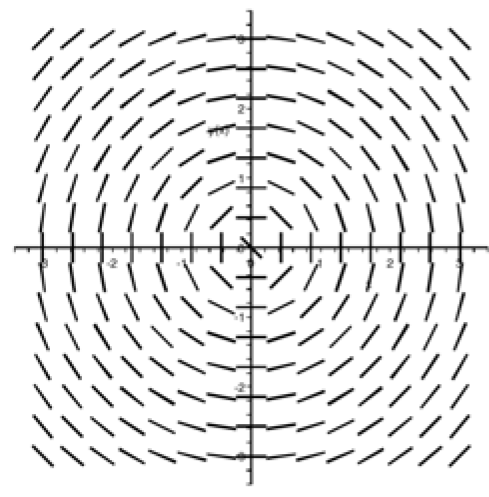
\includegraphics[width=3cm]{differentialgleichungen/rf1} & 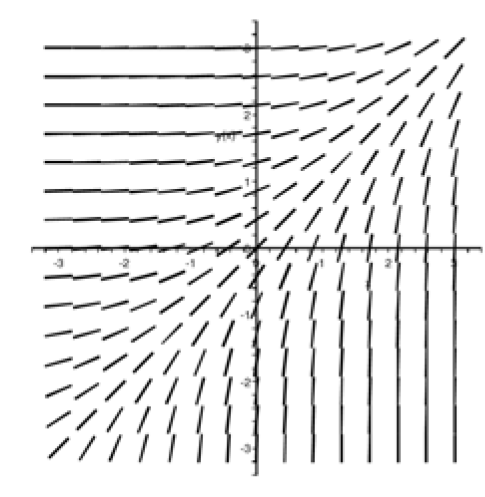
\includegraphics[width=3cm]{differentialgleichungen/rf2} & 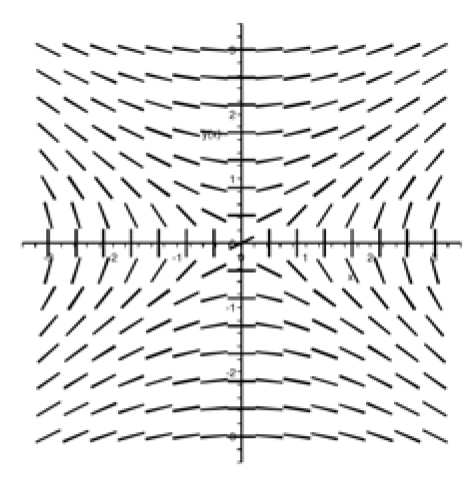
\includegraphics[width=3cm]{differentialgleichungen/rf3} & 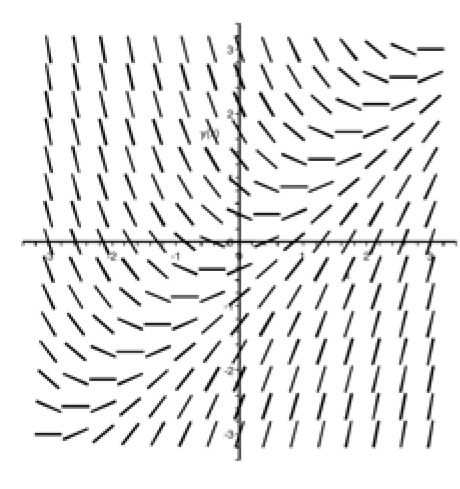
\includegraphics[width=3cm]{differentialgleichungen/rf4} & 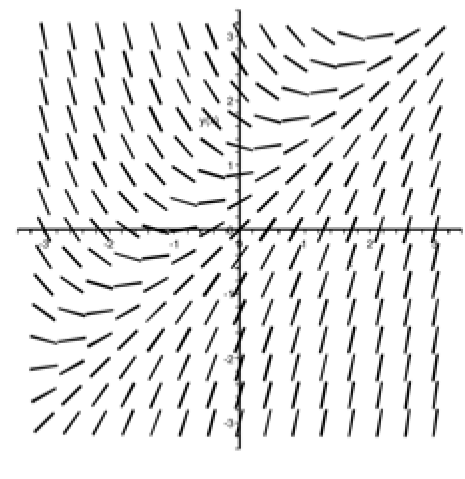
\includegraphics[width=3cm]{differentialgleichungen/rf5} & 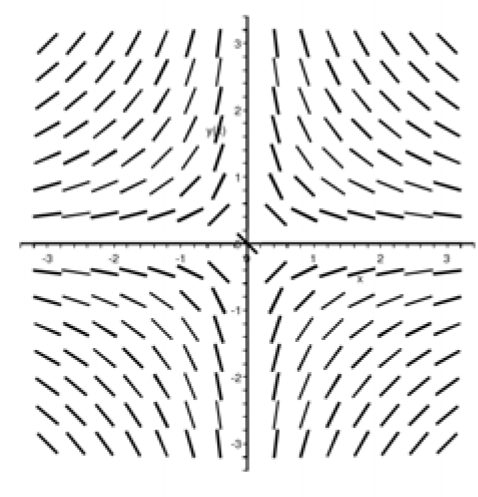
\includegraphics[width=3cm]{differentialgleichungen/rf6}\tabularnewline
\hline 
\hline 
$yy'+x=0$ & $y'=e^{x\text{−}y}$ & $2yy'=x$ & $y'=x\text{−}y$ & $y'=x\text{−}y+1$ & $y'x+y=0$\tabularnewline
\hline 
\end{tabular}


\subsection*{1.Ordnung}

$y'=f(x,y)=\frac{dy}{dx}$

$n'(t)=-\lambda\times n(t)$, allgemein löst $n(t)=C\times e^{-\lambda t}$
die DG


\subsubsection*{Trennen der Variablen}

$y'=f(x)\times g(y)=\frac{dy}{dx}$ jede Variable auf eine Seite,
dann getrennt Integrieren: $\int\frac{1}{g(y)}dy=\int f(x)dx+c$ 


\subsubsection*{Kurvenschaar-Problem}

Idee
\begin{enumerate}
\item Kurvenschaar $y=f(x,c)$, nach Konstante auflösen, dann in DG einsetzen
um C zu eliminieren
\item Zugehörige DG $y'=g(x,y)$
\item Zugehörige DG der orth. KS $y'=\frac{-1}{g(x,y)}$
\item Kurvenschaar bestimmen $y=f(x,c)$ 
\end{enumerate}

\subsubsection*{Beispiel}

Bestimmen Sie alle Kurven, die die Geraden durch den Nullpunkt rechtwinklig
schneiden.
\begin{enumerate}
\item Kurvenschar: $y=k\cdot x\Rightarrow k=\frac{y}{x}$
\item DG: $y'=k\Rightarrow y'=\frac{y}{x}$
\item Orth. Kurvenschar: $y'=-\frac{x}{y}$
\item Umformen: $\frac{dy}{dx}=-\frac{x}{y}\Rightarrow\int y\cdot dy=\int-x\cdot dx$
\item Integral Lösen und nach y auflösen
\end{enumerate}

\subsubsection*{Normalformen}

f(x) = Rechnung in x, g(y) = Rechnung in y
\begin{itemize}
\item $y'=f(x)+g(y)$ 1. Fall
\item $y'=f(x)\cdot g(y)$ 2. Fall
\end{itemize}

\subsubsection*{Integration durch Substitution}

1. Fall
\begin{itemize}
\item $y'=f(ax+by+c)$
\item $u=ax+by(x)+c$ => $y'=f(u)$, $u'=a+by'(x)$
\item in $u'$ für $y'$ die ursprüngliche Gleichung $y'=f(u)$ einsetzen
\end{itemize}
Beispiel
\begin{itemize}
\item $y'=x+y$
\item $u=x+y$
\item $u'=1+y'=1+u$
\item $\frac{du}{dx}=1+u$
\item $\int\frac{1}{1+u}\cdot du=\int dx\Rightarrow ln(1+u)=x+c\Rightarrow1+u=k\cdot e^{x}$
\item $1+x+y=k\cdot e^{x}\Rightarrow y=k\cdot e^{x}-x-1$
\end{itemize}
2. Fall
\begin{itemize}
\item $y'=f(\frac{y}{x})$ => $y'=f(u)$
\item $u=\frac{y}{x}$, $u(x)\times x=y$ => $u'(x)\times x+u(x)=y'$
\item $y'=u'x+u$ in $y'=f(u)$ eingesetzt und aufgelöst ergibt: $u'=\frac{1}{x}(f(u)-u)$
(anschliessend trennen der Variablen)
\end{itemize}
Beispiel:
\begin{itemize}
\item DG: $y'=\frac{3y^{2}+xy}{x^{2}}=3(\frac{y}{x})^{2}+\frac{y}{x}$
\item $u=\frac{y}{x}\Rightarrow f(u)=3u^{2}+u$
\item $u'=\frac{1}{x}\cdot(f(u)-u)=\frac{1}{x}\cdot(3u^{2}+u-u)=\frac{1}{x}\cdot u^{2}$
\item $\frac{du}{dx}=\frac{1}{x}\cdot u^{2}$
\item $\int\frac{1}{u2}=\int\frac{1}{x}$
\item Integral lösen, nach u auflösen und u einsetzen, danach nach y auflösen
\end{itemize}

\subsection*{2.Ordnung}

$x''(t)=-g$ 
\begin{itemize}
\item $x'(t)=-gt+v_{0}$
\item $x(t)=-gt^{2}\frac{1}{2}+v_{0}t+s_{0}$ => allgemeine Lösung
\item $v(0)=0,s(0)=0$ => $x(t)=-gt^{2}\frac{1}{2}$
\end{itemize}

\subsection*{Linerare DG (1.O)}

Normalformen
\begin{itemize}
\item $y'+f(x)\times y=g(x)$ -> inhomohene DG 1.O
\item $y'+f(x)\times y=0$ -> homogene DG 1.O
\end{itemize}
Allgemeine lösung mit freiem Parameter einer \textbf{Homogenen DG}
(durch trennen der Variabeln)
\begin{itemize}
\item $y_{h}(x)=K\times e^{-\int f(x)dx}$
\end{itemize}
Lösung einder \textbf{Inhomogenen DG}
\begin{enumerate}
\item LDG als homogene lösen -> $y_{h}$
\item $y_{p}=K(x)\times e^{-\int f(x)dx}$

\begin{enumerate}
\item $K'(x)=\frac{g(x)}{y_{h}(x)_{K=1}}$ bestimmen, danach Integrieren
\end{enumerate}
\item Allgemeine Lösung: $y_{a}(x)=y_{h}(x)+y_{p}(x)$ 
\item Falls Anfangsbedingungen vorhanden, einsetzen und partikuläre Lösung
bestimmen\end{enumerate}

